\begin{frame}{Ceph - What is it}
\begin{figure}[h]
    \centering
    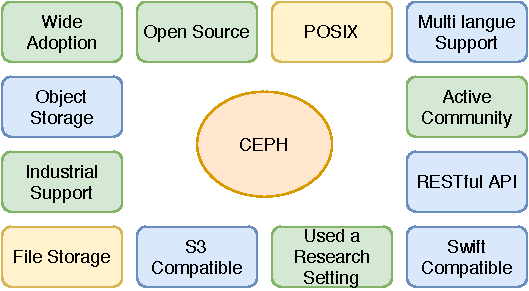
\includegraphics[width=\linewidth]{img/what-is-ceph.pdf}
\end{figure}
\end{frame}
\note{So Ceph is essence is Open Source scale-able distributed storage platform, that be used as a POSIX File System, Object store or Block device. It is S3 and Swift Compatible and has a a restful API that is implemented in multiple languages including Python,C++ and Java. It is approximately 14 years old and started as PhD project however has since been acquired by Redhat. It has many industrial and research facilities that use it, including STFC, CERN, OCADO and BLOOMBERG}
\begin{frame}{Ceph - Why is Diamond Interested}
\begin{block}{Reasons}
\begin{itemize}
        \item File \& Object Storage
        \item Open Source
        \item Scales
        \item Cloud integration
\end{itemize}
\end{block}
\end{frame}
\note{Now you make wonder why are interested in it for File storage when we deal with unstructured data, that because there is a lot of change that would be required some of which is already happening before we would go to full object store. }
